\documentclass[a4paper,oneside,12pt]{extreport}

\usepackage{mmap}
\usepackage[T2A]{fontenc}
\usepackage[utf8]{inputenc}
\usepackage[english,russian]{babel}

\usepackage[left=30mm, right=15mm, top=20mm, bottom=20mm]{geometry}

\setlength{\parindent}{1.25cm} % Абзацный отступ

\usepackage{setspace}
\onehalfspacing % Полуторный интервал

\frenchspacing % Равномерные пробелы
\usepackage{indentfirst} % Красная строка

\usepackage{microtype}
\sloppy

\usepackage{titlesec}
\titlespacing*{\chapter}{0pt}{-30pt}{8pt}
\titlespacing*{\section}{\parindent}{*4}{*4}
\titlespacing*{\subsection}{\parindent}{*4}{*4}
\titleformat{\chapter}{\LARGE\bfseries}{\thechapter}{20pt}{\LARGE\bfseries}
\titleformat{\section}{\Large\bfseries}{\thesection}{40pt}{\Large\bfseries}

\usepackage{graphicx}
\usepackage{caption}

\usepackage[unicode,pdftex]{hyperref}
\hypersetup{hidelinks}

\usepackage{amsmath}

%% title begin
\usepackage{wrapfig}

\makeatletter
	\def\vhrulefill#1{\leavevmode\leaders\hrule\@height#1\hfill \kern\z@}
\makeatother
%% title end

%% begin code
\usepackage{listings}
\usepackage{xcolor}

\lstset{
	basicstyle=\footnotesize\ttfamily,
	breakatwhitespace=true,
	breaklines=true,
	commentstyle=\color{gray},
	frame=single,
	keywordstyle=\color{blue},
	stringstyle=\color{red},
	tabsize=8
}

\newcommand{\code}[1]{\texttt{#1}}
%% end code


\begin{document}

\begin{titlepage}
	{\large % 14pt instead of 12pt
	\onehalfspacing
	\centering

	\begin{wrapfigure}[7]{l}{0.14\linewidth}
		\vspace{3mm}
		\hspace{-10mm}
		
\includegraphics[width=0.93\linewidth]{inc/img/bmstu-logo}
	\end{wrapfigure}
	{\singlespacing \footnotesize \bfseries Министерство науки и высшего образования Российской Федерации\\Федеральное государственное бюджетное образовательное учреждение\\высшего образования\\<<Московский государственный технический университет\\имени Н.~Э.~Баумана\\ (национальный исследовательский университет)>>\\(МГТУ им. Н.~Э.~Баумана)\\}

	\vspace{-2.2mm}
	\vhrulefill{0.9mm}\\
	\vspace{-7.5mm}
	\vhrulefill{0.2mm}\\
	\vspace{2mm}

	{\doublespacing \small \raggedright ФАКУЛЬТЕТ \hspace{37mm} «Информатика и системы управления»\\
	КАФЕДРА \hspace{17mm} «Программное обеспечение ЭВМ и информационные технологии»\\}

	\vspace{30mm}

	\textbf{ОТЧЁТ}\\
	По лабораторной работе № 2\\
	По курсу: «Моделирование»\\
	Тема: «Распределение случайных величин»\\
	Вариант: 6 $\equiv$ 2 (mod 4)\\

	\vspace{40mm}

	\begin{flushleft}
		\begin{tabular}{lr}
			\textbf{Студент:}        & Керимов~А.~Ш. \\
			\textbf{Группа:}         & ИУ7-74Б       \\
			\textbf{Оценка (баллы):} & \hrulefill    \\
			\textbf{Преподаватель:}  & Рудаков~И.~В. \\
		\end{tabular}
	\end{flushleft}

	\vfill

	Москва\\
	\the\year\\}
\end{titlepage}

\setcounter{page}{2}


\paragraph{Цель работы.} Получение навыков проведения исследований компьютерной математической модели, построенной на квазилинейном уравнении параболического типа.

Исследование проводится с помощью программы, созданной в лабораторной работе № 4.

\section*{Исходные данные}

\begin{enumerate}
	\item Значения параметров (все размерности согласованы)
	\begin{equation*}
		\begin{aligned}
			k(T) &= a_1(b_1 + c_1T^{m_1}) &\text{Вт/см К},\\
			c(T) &= a_2+b_2T^{m_2}-\frac{c_2}{T_2} &\text{Дж/см³ К}.
		\end{aligned}
	\end{equation*}
	\begin{equation*}
		\begin{aligned}
			a_1 &= 0,0134, & b_1 &= 1,                 & c_1 &= 4,35\cdot10^{-4}, & m_1 &= 1,\\
			a_2 &= 2,049,  & b_2 &= 0,563\cdot10^{-3}, & c_2 &= 0,528\cdot10^5,   & m_2 &= 1.
		\end{aligned}
	\end{equation*}
	\begin{equation*}
		\begin{aligned}
			\alpha(x) &= \frac{c}{x-d}, &                 \\
			\alpha_0  &= 0,05           & \text{Вт/см² К},\\
			\alpha_N  &= 0,01           & \text{Вт/см² К},\\
			l         &= 10             & \text{см},      \\
			T_0       &= 300            & \text{К},       \\
			R         &= 0,5            & \text{см}.
		\end{aligned}
	\end{equation*}

	 \item Поток тепла
	\begin{equation*}
	F(t) = \frac{F_{\max}}{t_{\max}} \cdot t \cdot \exp{\left(1 - \frac{t}{t_{\max}}\right)},
	\end{equation*}

	где $F_{\max}$ — амплитуда импульса потока, $t_{\max}$ — время достижения амплитуды.
\end{enumerate}

\pagebreak
\section*{Результаты работы}

\begin{enumerate}
	\item \textbf{Провести исследование по выбору оптимальных шагов по времени $\tau$ и пространству $h$. Шаги должны быть максимально большими при сохранении устойчивости разностной схемы и заданной точности расчета.}

	Оценим точность расчёта, уменьшая шаги и наблюдая сходимость решений, как это делалось в \href{ftp://eufs.bmstu.ru/19426610-bd1a-11e6-93f1-005056960017/27-03-2020-%D0%97%D0%B0%D0%B4%D0%B0%D0%BD%D0%B8%D0%B5_%D0%BD%D0%B0_%D0%BB%D0%B0%D0%B1_%D1%80%D0%B0%D0%B1_%E2%84%961.doc}{ЛР1}.

	\begin{figure}[H]
		\centering
		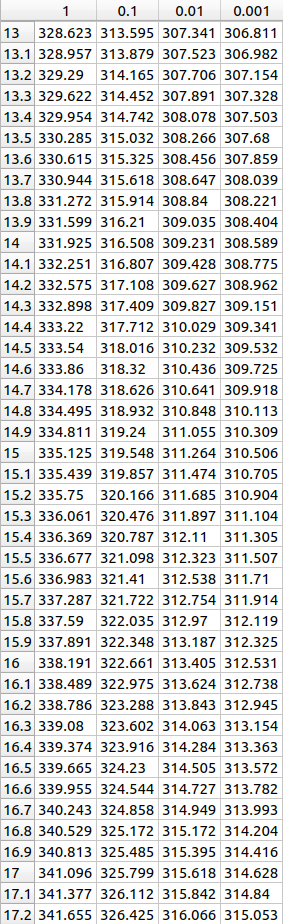
\includegraphics[height=0.5\textheight]{inc/img/steph.png}
		\hspace{1cm}
		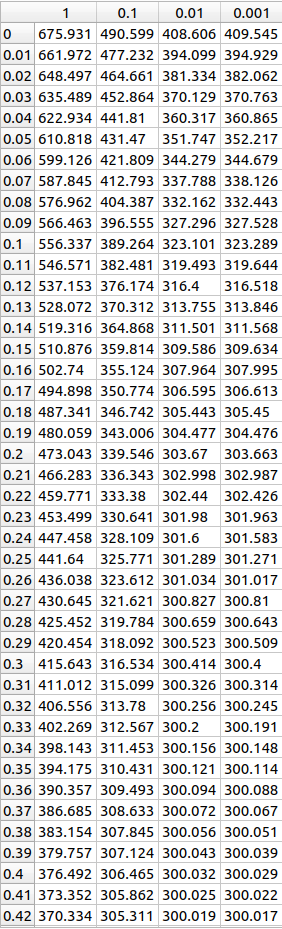
\includegraphics[height=0.5\textheight]{inc/img/steptau10.png}
		\hspace{1cm}
		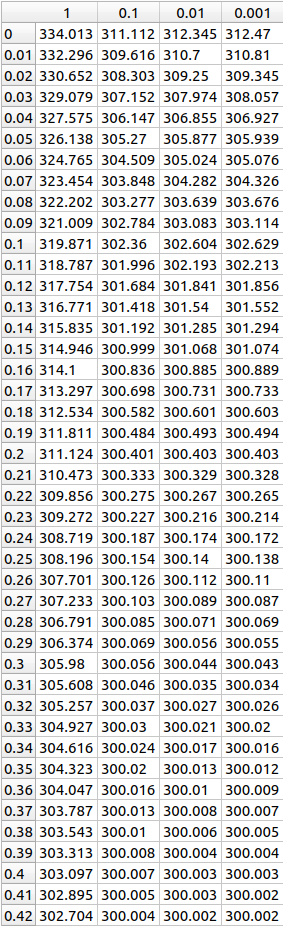
\includegraphics[height=0.5\textheight]{inc/img/steptau100.png}
		\caption{Шаг в пространстве (слева), по времени при $t_{\max} = 10$ (в центре), $t_{\max} = 100$ (справа)}
		\label{img:step}
	\end{figure}

	В первой таблице указаны температуры на расстоянии 1 см от времени, указанном в первой колонке, в зависимости от шага по пространству, указанного в первой строке.
	Во второй и третьей таблицах указаны температуры спустя секунду на расстоянии, указанном в первом столбце, в зависимости от шага по времени, указанного в первой строке.

	Видно, что при следующим за $0,01$ шагом значения практически совпадают, следовательно, оптимальный шаг по пространству — $h = 0,01$.

	Аналогично, оптимальный шаг по времени при $t_{\max} = 10$ — $\tau = 0,01$, при $t_{\max} = 100$ — $\tau = 0,1$.
	Видно, что оптимальный шаг зависит от времени достижения амплитуды $t_{\max}$, приближённо можно считать, что на 3 порядка её меньше.

	Рассмотрим влияние на результат амплитуды импулься и времени её достижения (рисунки \ref{img:xn100-10}–\ref{img:xn500-100}).
	Очевидно, что с ростом $F_{\max}$ возрастает максимальная температура стержня, а при изменении $t_{\max}$ меняется время достижения точки с максимальной температурой.

	\begin{figure}[H]
		\centering
		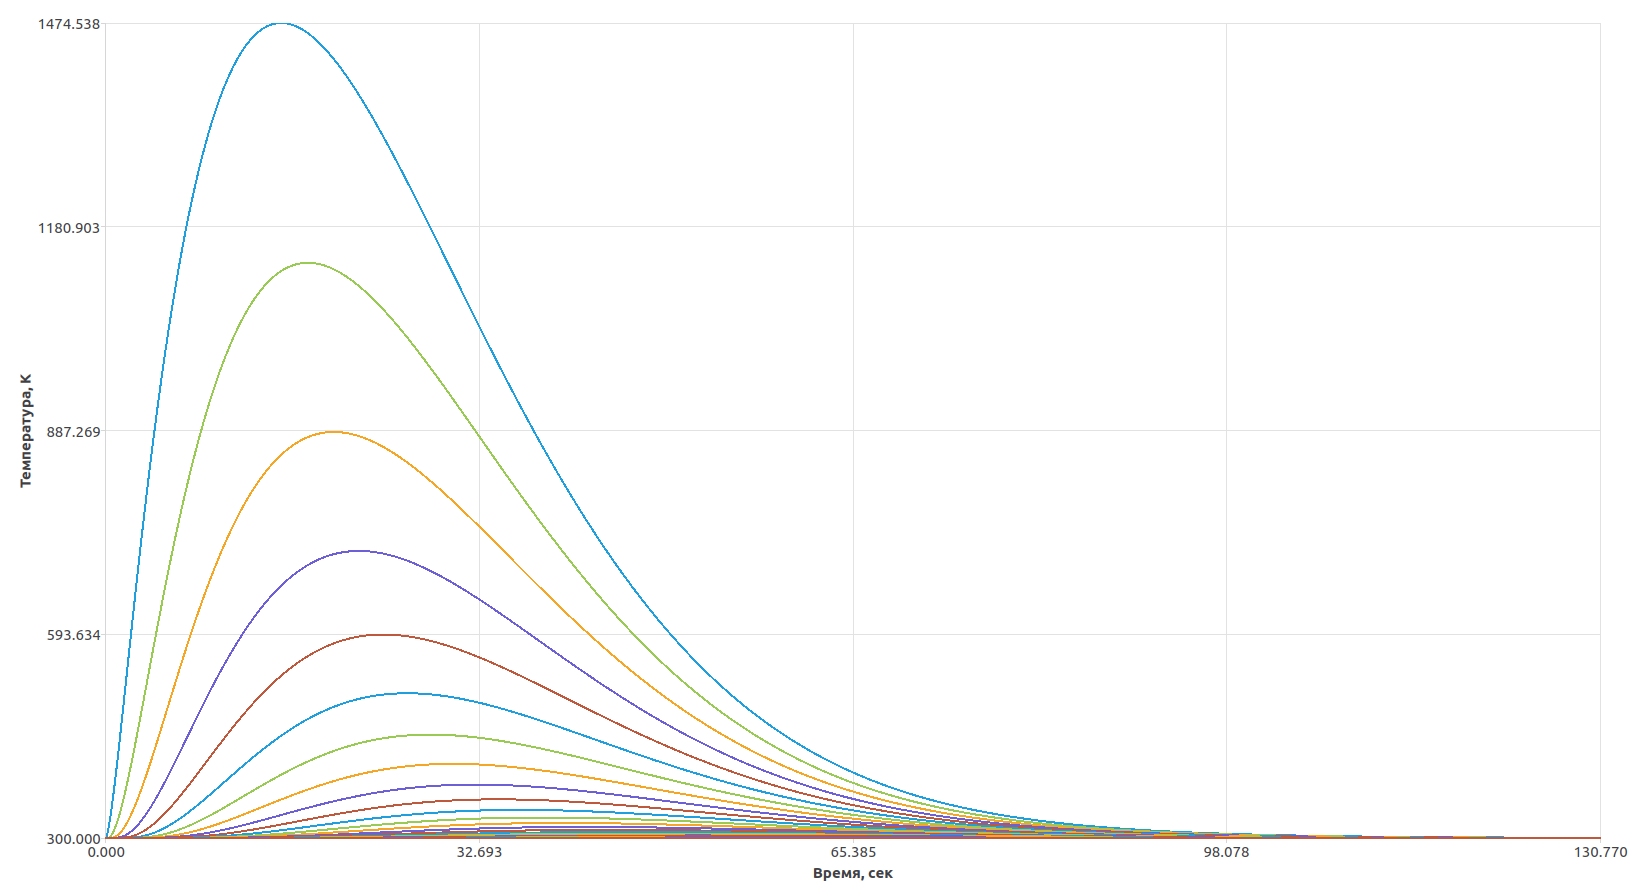
\includegraphics[width=0.75\linewidth]{inc/img/xn100-10.png}
		\caption{График $(x_n, t)$ при $F_{\max} = 100,\ t_{\max} = 10$}
		\label{img:xn100-10}
	\end{figure}

	\begin{figure}[H]
		\centering
		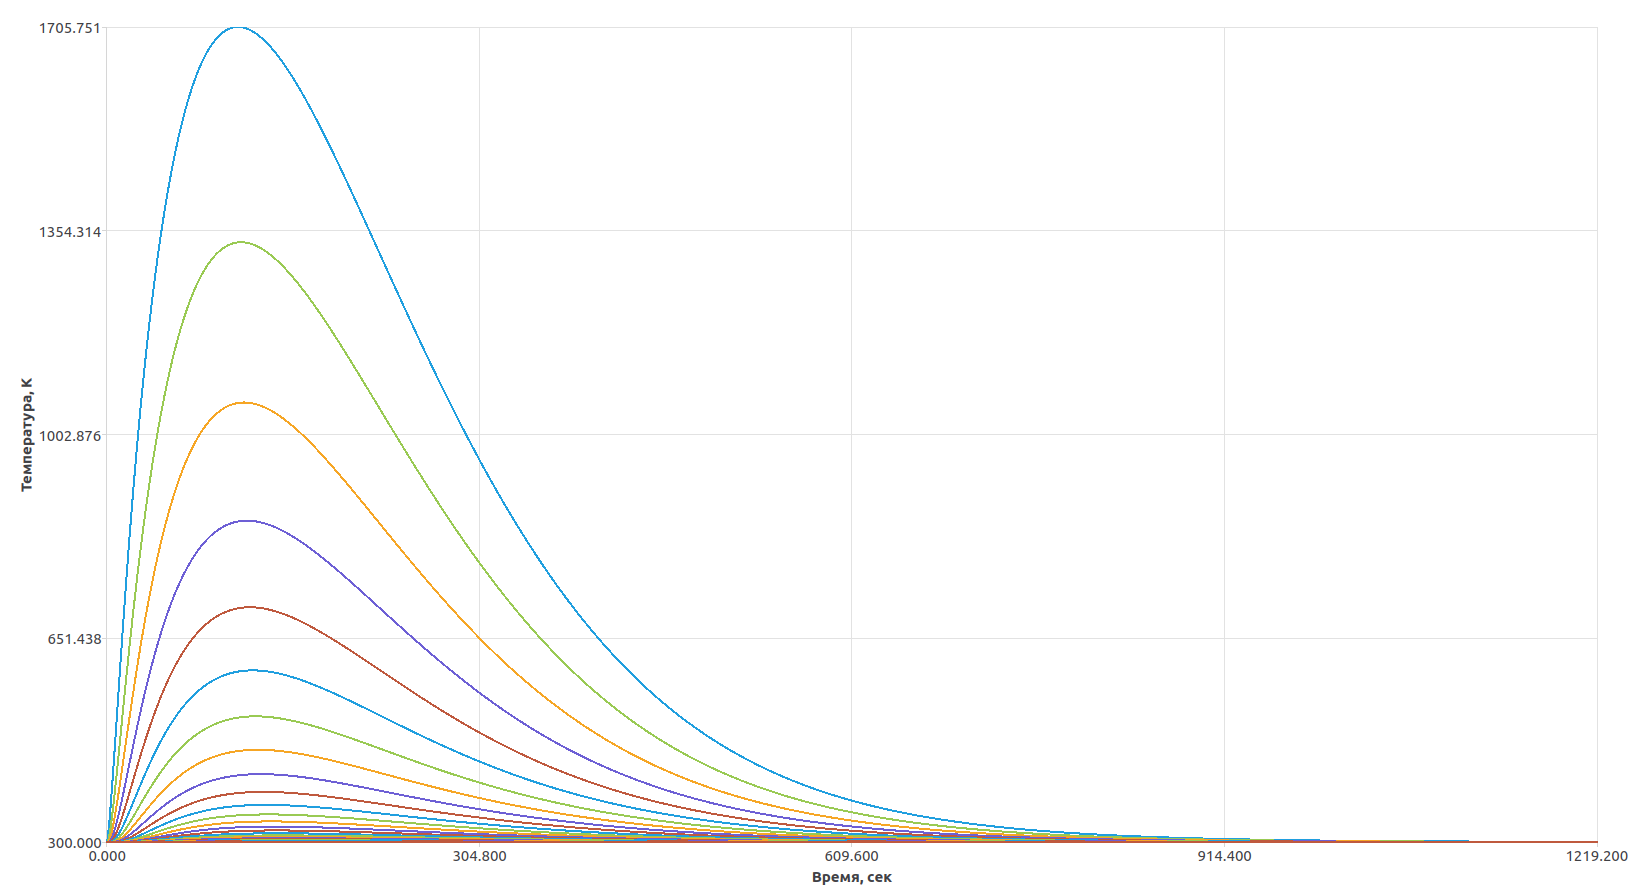
\includegraphics[width=0.75\linewidth]{inc/img/xn100-100.png}
		\caption{График $T(x_n, t)$ при $F_{\max} = 100,\ t_{\max} = 100$}
		\label{img:xn100-100}
	\end{figure}

	\begin{figure}[H]
		\centering
		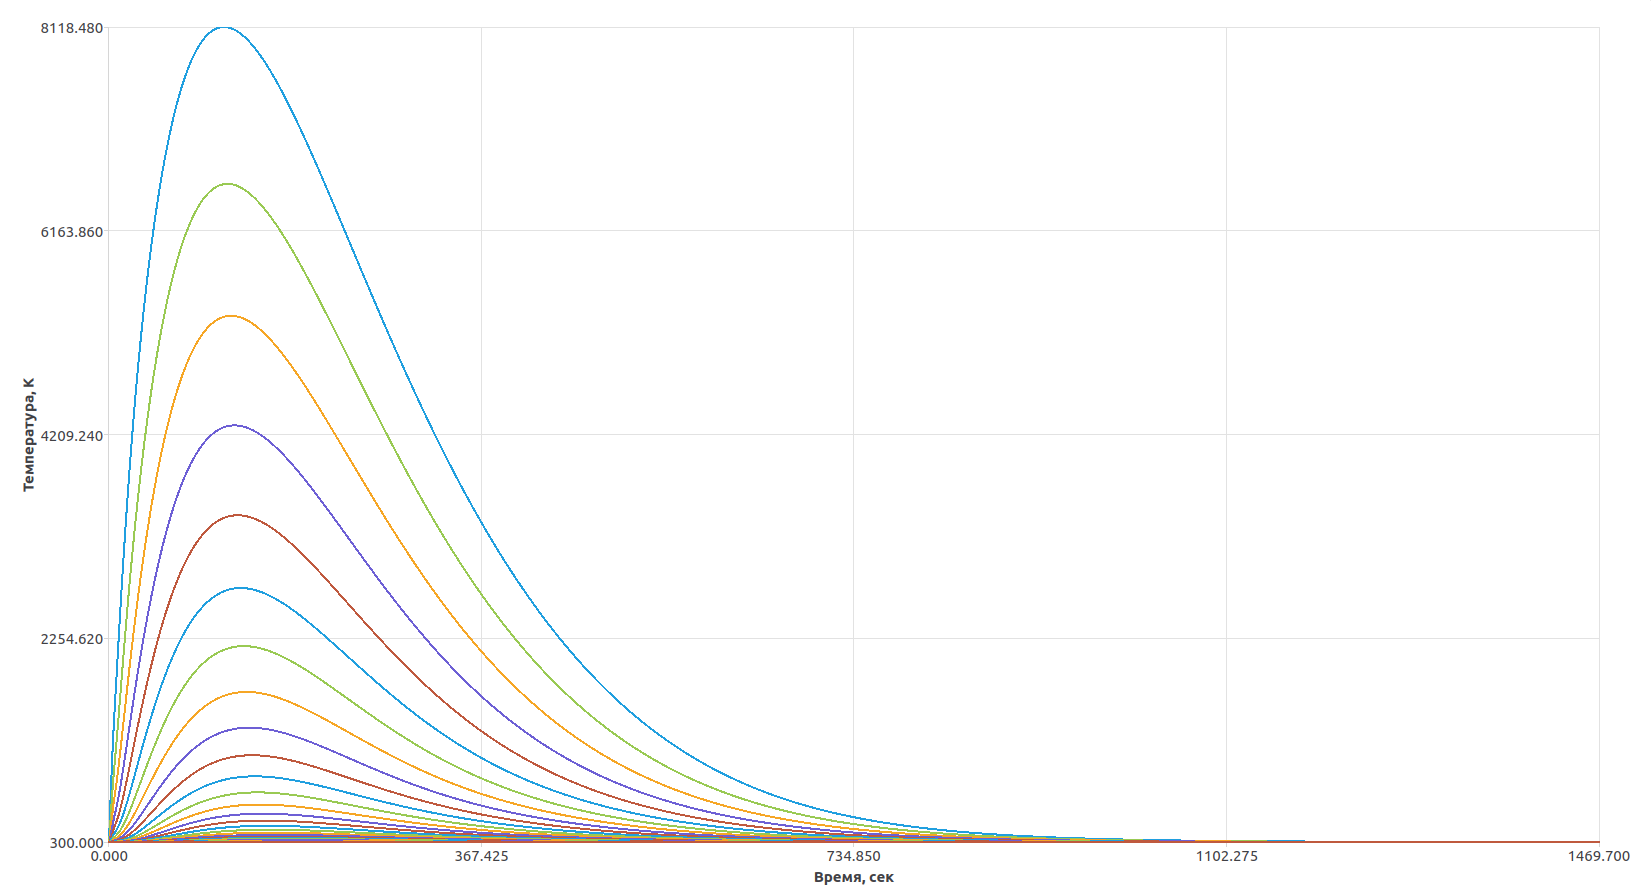
\includegraphics[width=0.75\linewidth]{inc/img/xn1000-100.png}
		\caption{График $T(x_n, t)$ при $F_{\max} = 1000,\ t_{\max} = 100$}
		\label{img:xn500-100}
	\end{figure}


	\item \textbf{График зависимости температуры $T\left(0, t\right)$ при 3–4 значениях параметров $a_2$ и/или $b_2$ теплоемкости.}

	\begin{equation*}
		\begin{aligned}
			a_{20} &= 2,049,    & a_{21} &= 5,     & a_{22} &= 10,   & a_{23} &= 15,  \\
			b_{20} &= 0,000564, & b_{21} &= 0,001, & b_{22} &= 0,01, & b_{23} &= 0,1. \\
		\end{aligned}
	\end{equation*}
	\begin{figure}[H]
		\centering
		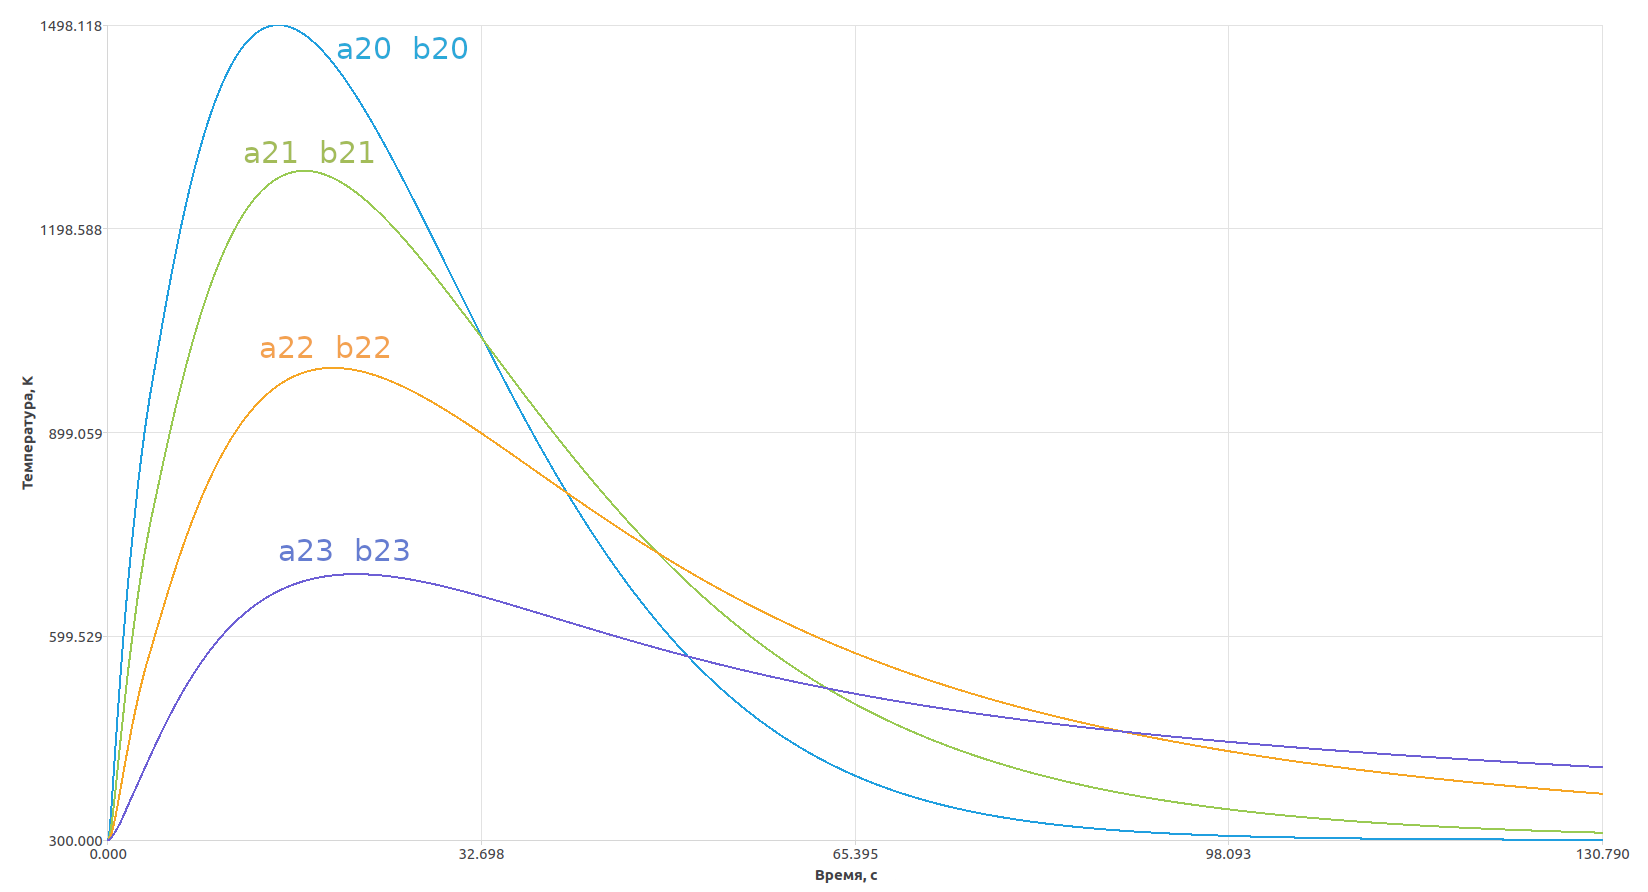
\includegraphics[width=0.75\linewidth]{inc/img/capacity.png}
		\caption{График $T\left(0, t \right)$ при разных значениях $a_2$, $b_2$}
		\label{img:capacity}
	\end{figure}

	С ростом теплоемкости темп нарастания температуры снижается.

	\item \textbf{График зависимости температуры $T(0, t)$ (т. е. при $x = 0$) в частотном режиме теплового нагружения. Импульсы следуют один за другим с заданной частотой $\nu$ (частота определяется количеством импульсов в 1 секунду).}

	На рисунках \ref{img:impulse1}–\ref{img:impulse4} видно, что при увеличении частоты размах колебаний температуры уменьшается вплоть до нуля, т.~е. реализуется квазистационарный режим.

	\begin{figure}[H]
		\centering
		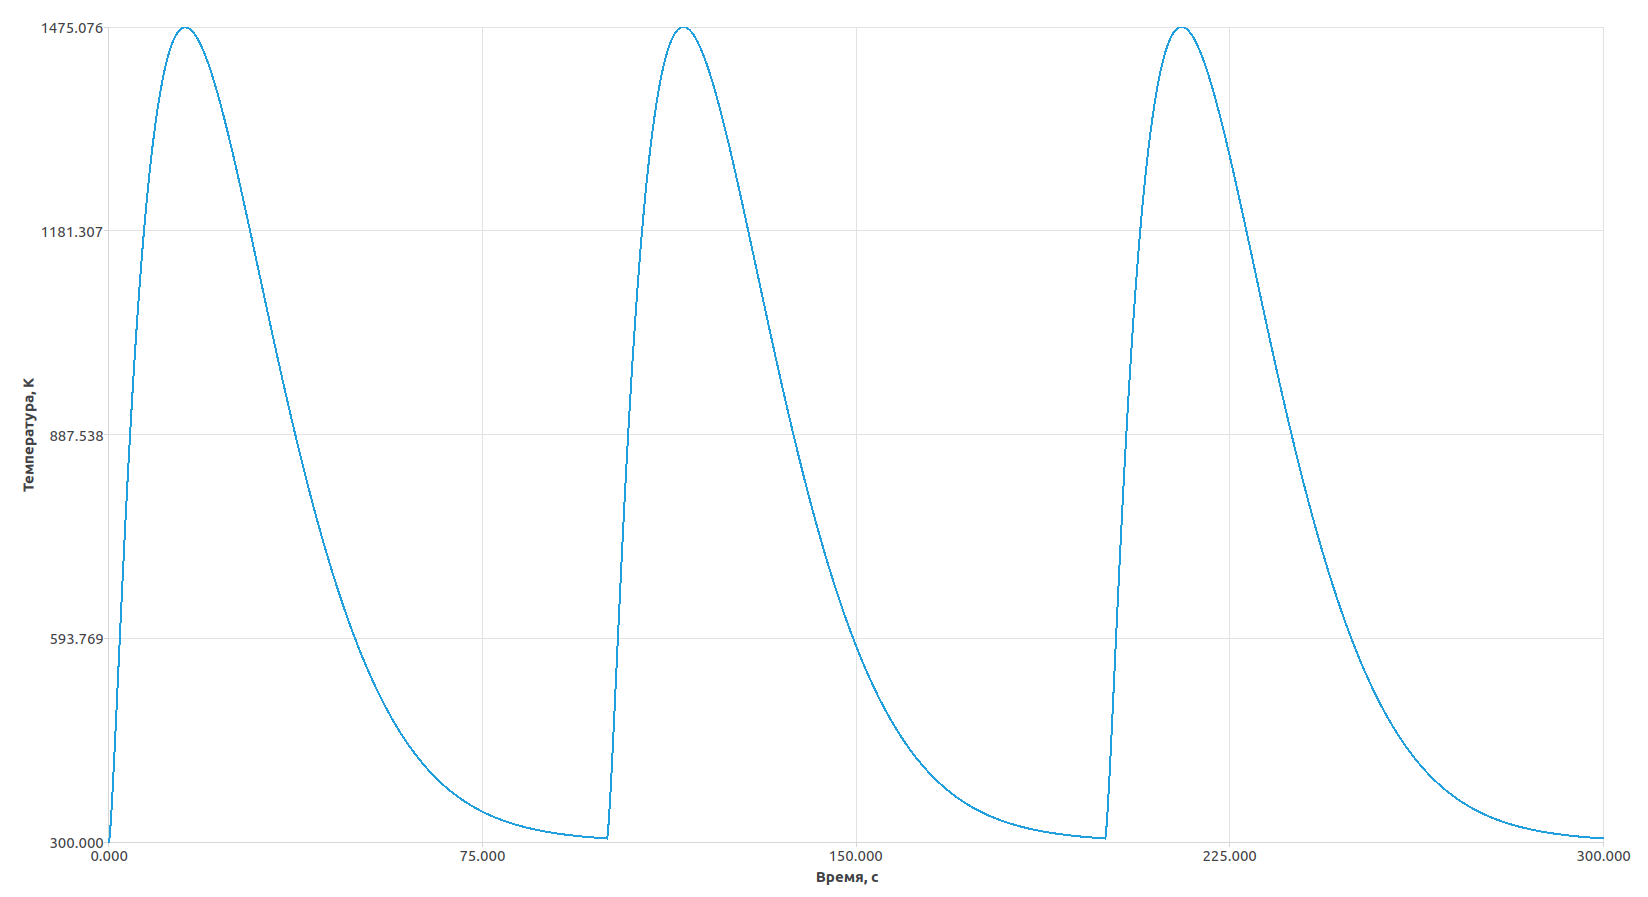
\includegraphics[width=0.75\linewidth]{inc/img/impulse1.png}
		\caption{Частота $\nu = 0,01$}
		\label{img:impulse1}
	\end{figure}

	\begin{figure}[H]
		\centering
		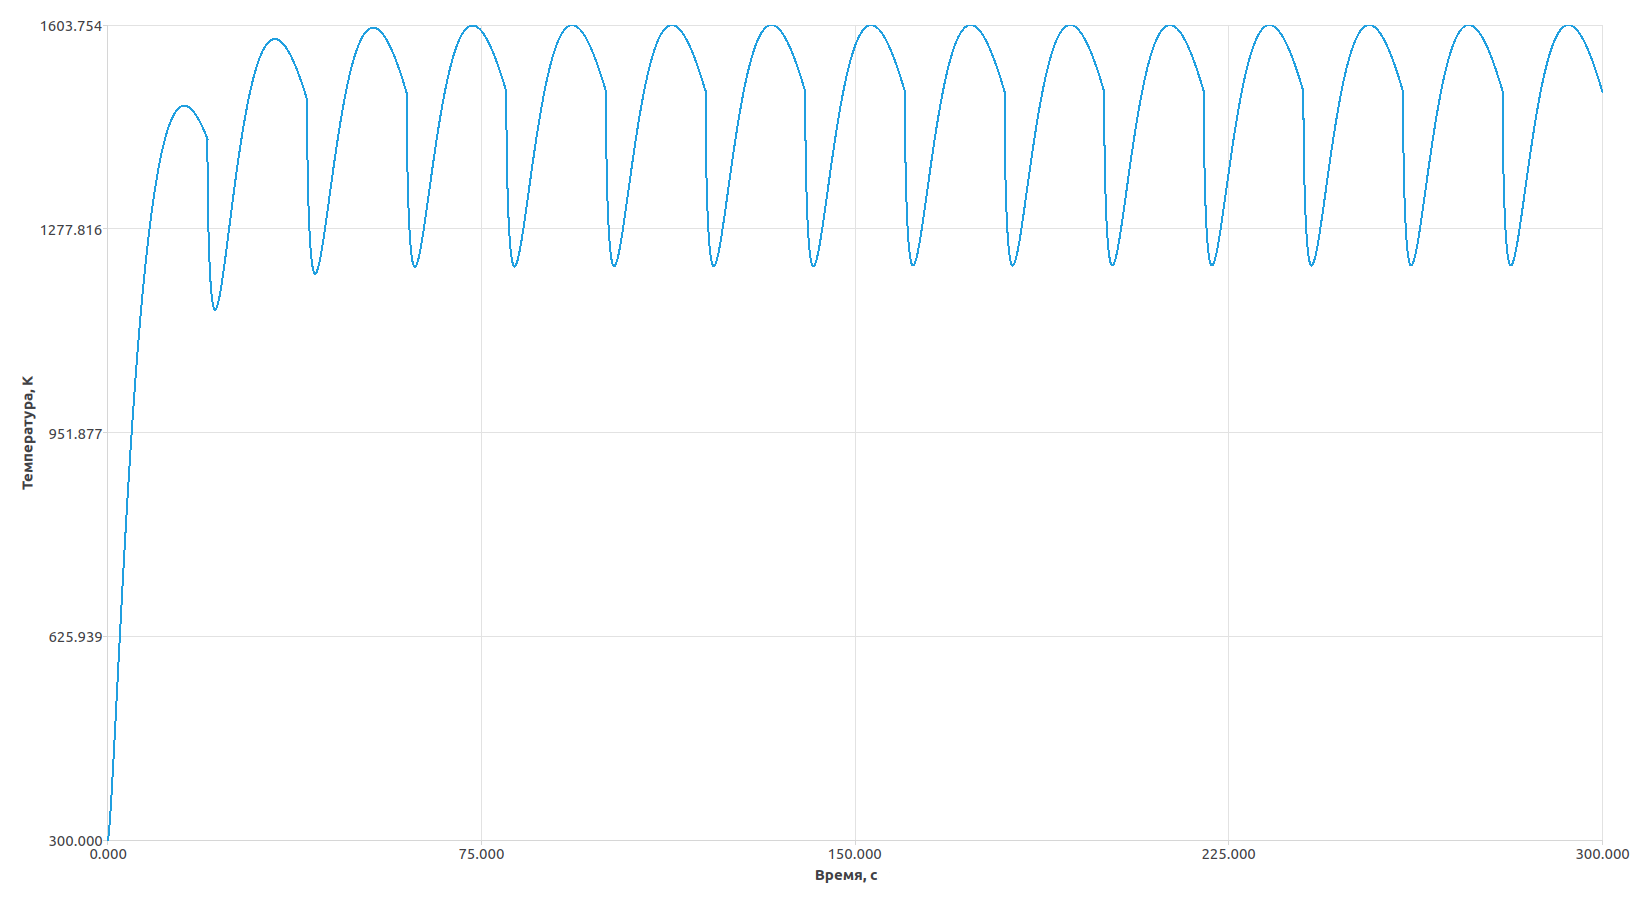
\includegraphics[width=0.75\linewidth]{inc/img/impulse2.png}
		\caption{Частота $\nu = 0,05$}
		\label{img:impulse2}
	\end{figure}

	\begin{figure}[H]
		\centering
		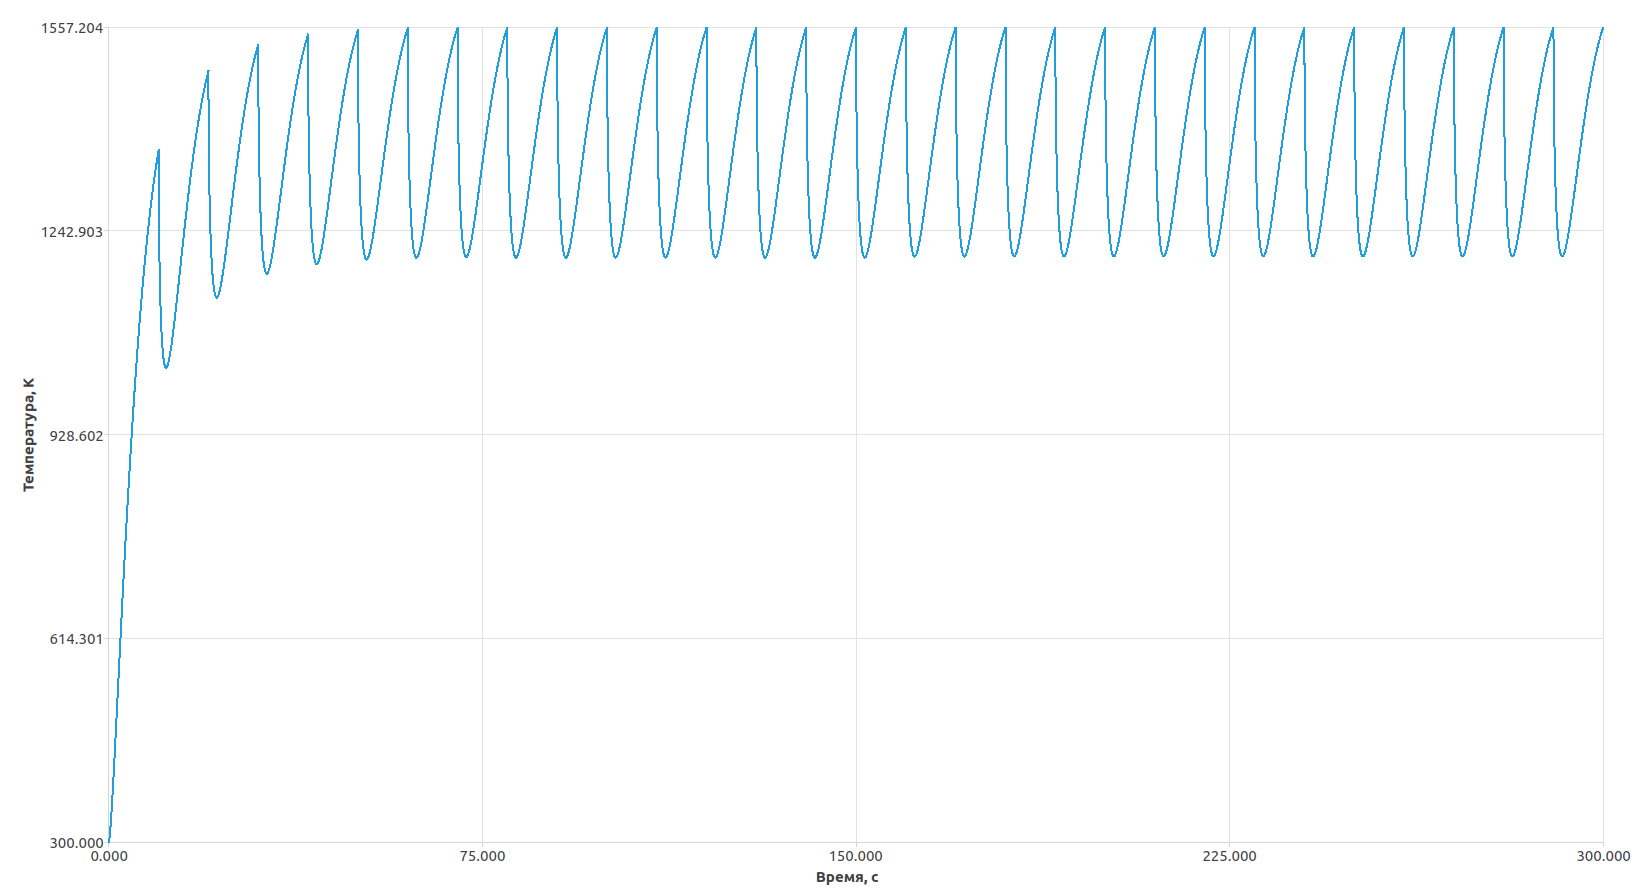
\includegraphics[width=0.75\linewidth]{inc/img/impulse3.png}
		\caption{Частота $\nu = 0,1$}
		\label{img:impulse3}
	\end{figure}

	\begin{figure}[H]
		\centering
		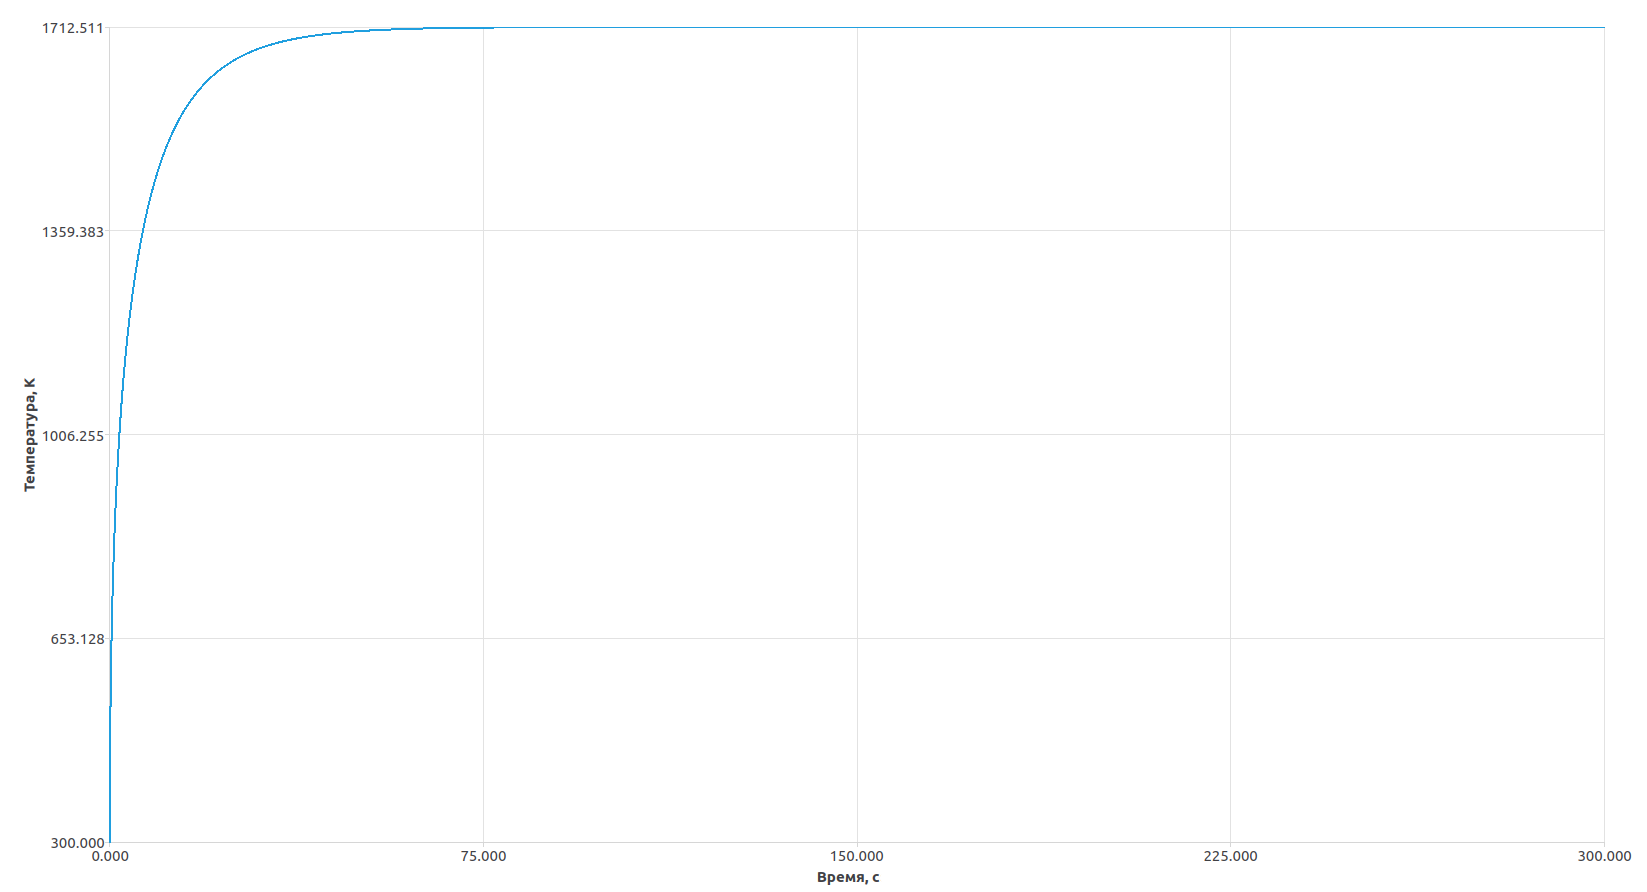
\includegraphics[width=0.75\linewidth]{inc/img/impulse4.png}
		\caption{Частота $\nu = 100$}
		\label{img:impulse4}
	\end{figure}

	Полученное температурное поле совпадает с результатом расчёта по программе из ЛР3 при всех одинаковых параметрах модели.
	На рисунке \ref{img:lab_03} график, полученный программой из ЛР3, а на рисунке \ref{img:lab_03_new} — из текущей.

	\begin{figure}[H]
		\centering
		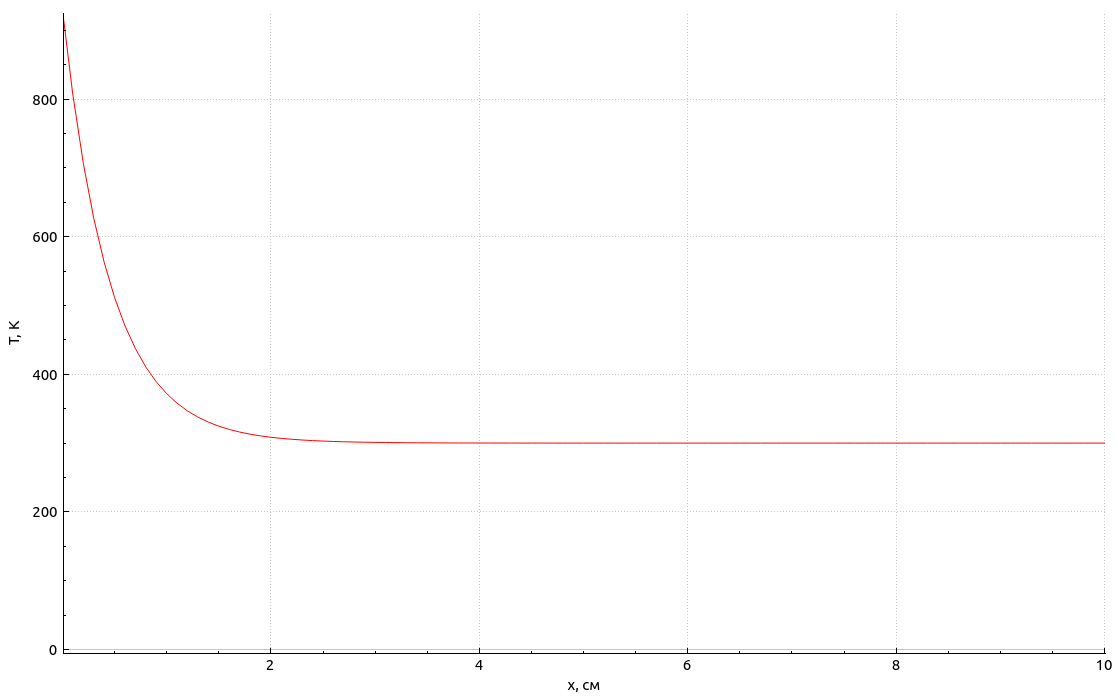
\includegraphics[width=\linewidth]{inc/img/lab03.png}
		\caption{График из ЛР3}
		\label{img:lab_03}
	\end{figure}

	\begin{figure}[H]
		\centering
		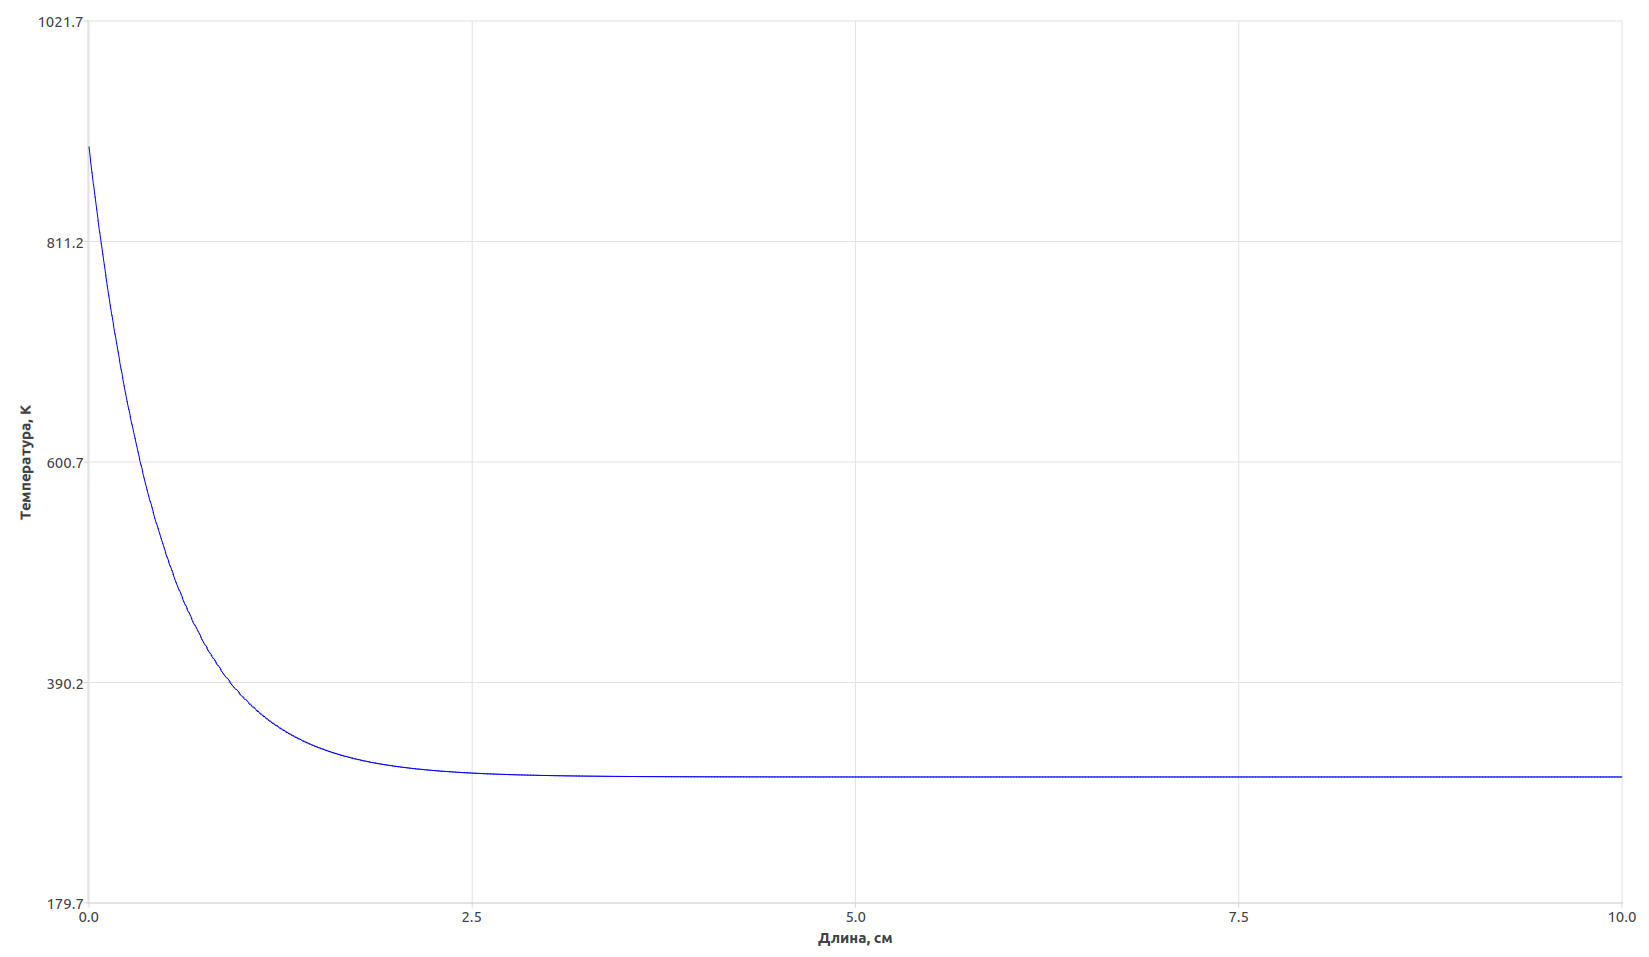
\includegraphics[width=\linewidth]{inc/img/lab03_new.png}
		\caption{График из текущей ЛР}
		\label{img:lab_03_new}
	\end{figure}
\end{enumerate}

\end{document}
